\usetikzlibrary{arrows}
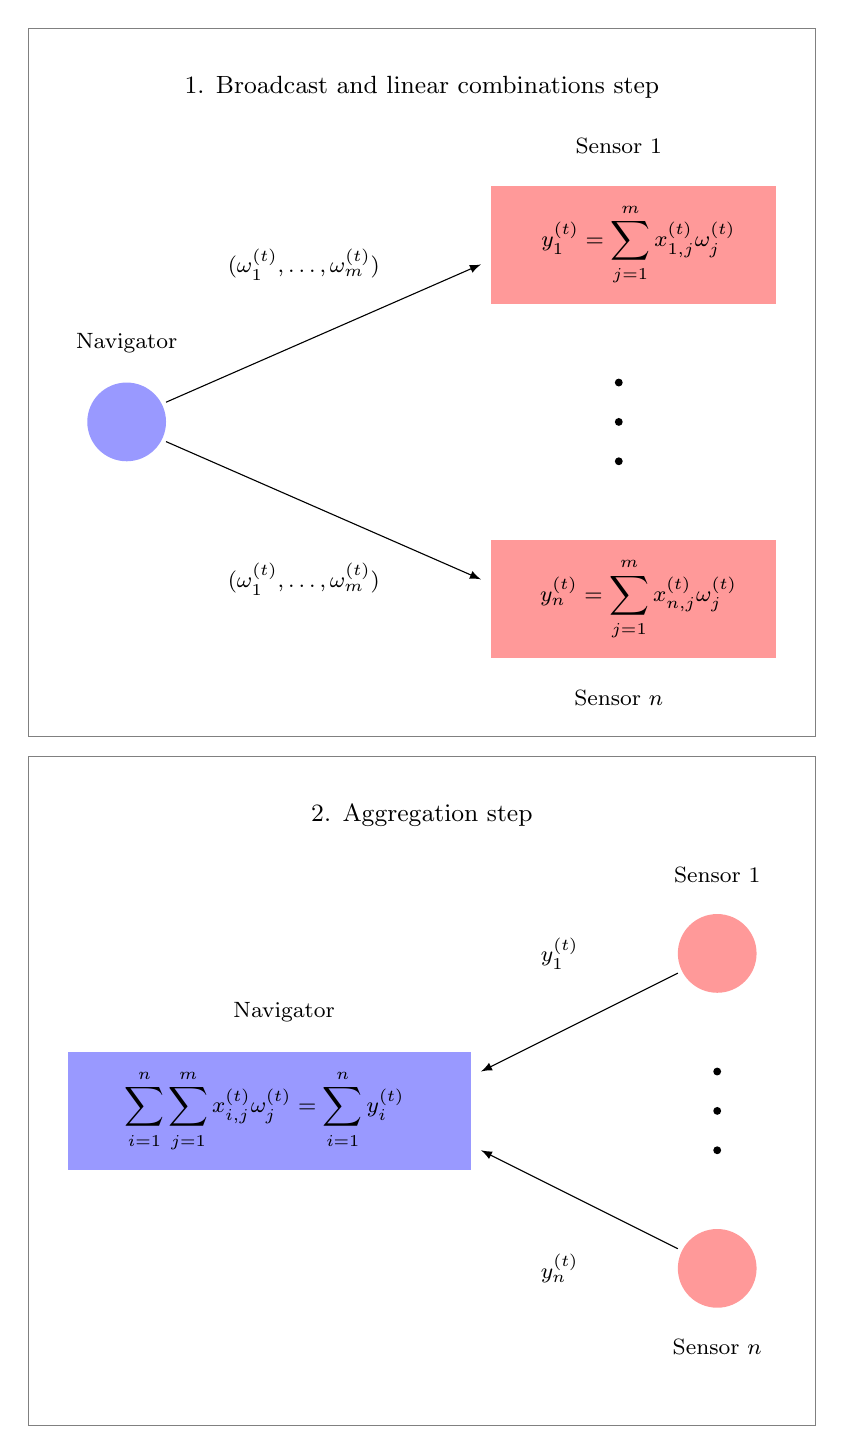
\begin{tikzpicture}[font=\footnotesize]
    % Step 1
    \node at (5,22.5) {\small 1. Broadcast and linear combinations step};
    % Navigator
    \node at (1.25,19.25) {Navigator};
    \fill (1.25,18.25) [blue!40] ellipse (0.5 and 0.5);
    % Sensors
    \node at (7.5,21.75) {Sensor $1$};
    \fill [red!40] (5.875,19.75) rectangle (9.5,21.25);
    \node at (7.75,20.5) {$\displaystyle y_1^{(t)} = \sum^m_{j=1}x_{1,j}^{(t)}\omega_j^{(t)}$};
    \node at (7.5,14.75) {Sensor $n$};
    \fill [red!40] (5.875,15.25) rectangle (9.5,16.75);
    \node at (7.75,16) {$\displaystyle y_n^{(t)} = \sum^m_{j=1}x_{n,j}^{(t)}\omega_j^{(t)}$};
    \fill [black] (7.5,18.75) circle (0.05);
    \fill [black] (7.5,17.75) circle (0.05);
    \fill [black] (7.5,18.25) circle (0.05);
    % Lines
    \draw [-latex] plot[smooth, tension=.7] coordinates {(1.75,18.5) (5.75,20.25)};
    \draw [-latex] plot[smooth, tension=.7] coordinates {(1.75,18) (5.75,16.25)};
    \node at (3.5,20.25) {$(\omega_1^{(t)},\dots ,\omega_m^{(t)})$};
    \node at (3.5,16.25) {$(\omega_1^{(t)},\dots ,\omega_m^{(t)})$};
    
    % Step 2
    \node at (5,13.25) {\small 2. Aggregation step};
    % Navigator
    \node at (3.25,10.75) {Navigator};
    \fill [blue!40] (0.5,8.75) rectangle (5.625,10.25);
    \node at (3,9.5) {$\displaystyle \sum^{n}_{i=1}\sum^{m}_{j=1} x_{i,j}^{(t)}\omega_j^{(t)} = \sum^n_{i=1}y^{(t)}_{i}$};
    % Sensors
    \node at (8.75,12.5) {Sensor $1$};
    \fill  (8.75,7.5) [red!40] ellipse (0.5 and 0.5);
    \node at (8.75,6.5) {Sensor $n$};
    \fill  (8.75,11.5) [red!40] ellipse (0.5 and 0.5);
    \fill [black] (8.75,10) circle (0.05);
    \fill [black] (8.75,9) circle (0.05);
    \fill [black] (8.75,9.5) circle (0.05);
    % Lines
    \draw [-latex] plot[smooth, tension=.7] coordinates {(8.25,11.25) (5.75,10)};
    \draw [-latex] plot[smooth, tension=.7] coordinates {(8.25,7.75) (5.75,9)};
    \node at (6.75,11.5) {$y_1^{(t)}$};
    \node at (6.75,7.5) {$y_n^{(t)}$};
    
    % Bounding rectangles
    \draw [gray] (0,23.25) rectangle (10,14.25);
    \draw [gray] (0,14) rectangle (10,5.5);
\end{tikzpicture}